% !TeX root = RJwrapper.tex
\title{Capitalized Title Here}
\author{by Author One, Author Two, and Author Three}

\maketitle

\abstract{%
Fisher do not only catch one species. They have a set of possible
choices, called `fishing portfolio'. Some species are easier to shift as
gear and method used are similar between them. Therefore, the cost of
shifting between species is low and fishers could adapt quickly to a
shift in fish species spatial distributions in response to climate
change. Nevertheless, it is not clear whether actually this substitution
happen as other constraint may be in play. Port constraints, as well as
market characteristics could reduce substitution between species. In
this study we analyze how changing in spatial distribution affects
landing subtitution between three coastal pelagic species: Pacific
sardine, market squid and Northern anchovy. We primary focus on the
substitution that ocur between these species, and we project change on
catch composition due to future climate change.
}

\hypertarget{introduction}{%
\section{Introduction}\label{introduction}}

Fishing portfolios are an important mechanism to safeguard fishers
livelihood. Diversification strategy have been principally associated to
reducing income variability. For instance, when a species abundance is
reduced due to environmental conditions, fisher can change the targeted
species. However, there is no always room for diversification. Switching
between species can be costly if gears are quite different between
species, or a new permit is required for legal fishing. Moreover, even
though fisher may have flexibility switching between species, port
infrastructure and markets may impose some restrictions on this
flexibility. Therefore, it is not clear how change in species
distribution would be reflected in landings.

In this study we analyze how changing in spatial distribution affects
landing substitutions between three coastal pelagic species (CPS):
Pacific sardine (PSDN), market squid (MSQD) and Northern anchovy (NANC).
Moreover, using climate projections we can predict how catch composition
is affected under climate change. Our analysis is focused on the US west
coast CPS fishery.

Our papers builds on the model developed by \citet{smith2021potential}
for sardine landings. We expand their research Fisheries historically
have been analyzed as single species. We expand their model including a
landing equation for all of the three species analyzed. Moreover, we use
the probability of presence obtained from Species Distribution Models
(SDM) as explanatory variable instead of landing by species. This allows
us to project landing over time using SDM predictions for different
climate scenarios. Additionally, we analyze how species distribution
interact between each others. We expect that this additions allows us to
characterize better how fishers portfolio is composed, and also to
understand better species interactions on catch rates.

The remainder of the paper is organized as follows: Section
\ref{coastal-pelagic-species-fishery} provides background on the CPS
fishery in the US west coast. In Section \ref{methods} we discusses our
data set and empirical strategy. Section \ref{results} presents the
results of the estimations, and we conclude in Section
\ref{conclusions}.

\hypertarget{coastal-pelagic-species-fishery}{%
\section{Coastal Pelagic Species
fishery}\label{coastal-pelagic-species-fishery}}

Before Pacific sardine closure in 2015, the CPS fishery have been mainly
dominated by Pacific sardine and market squid in landings (see Figure
\ref{fig:avg_lan_rev}). In terms of revenue, due to the low prices
received for sardine, the revenues in the CPS fishery are the highest
for market squid.

\begin{Schunk}
\begin{figure}
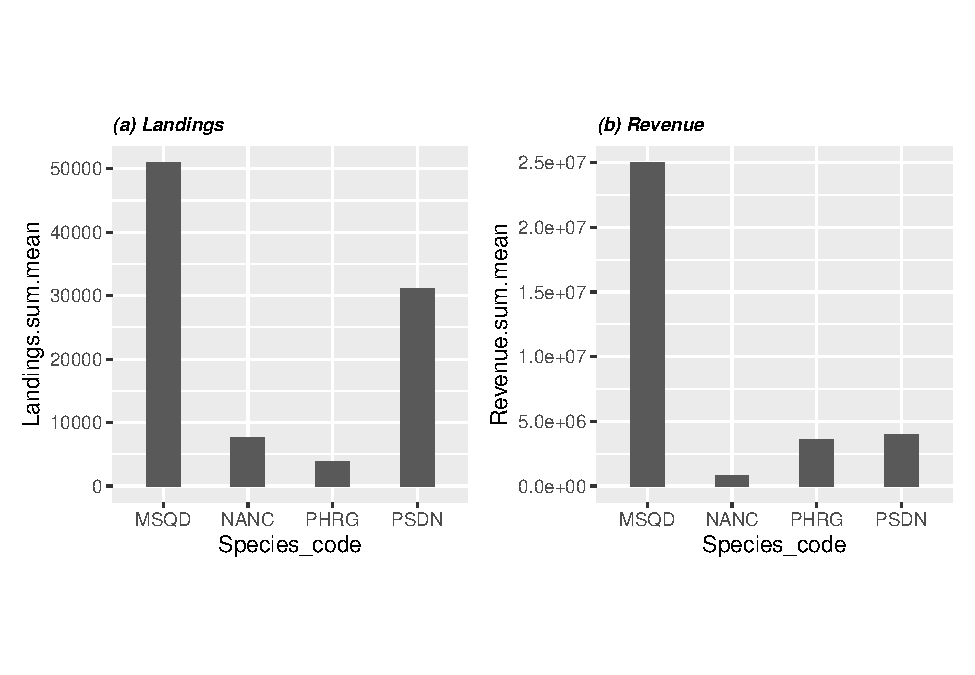
\includegraphics{econ_landings_paper_files/figure-latex/avg_landings-1} \caption{Average annual landing and revenues for the CPS fishery by species.\label{fig:avg_lan_rev}}\label{fig:avg_landings}
\end{figure}
\end{Schunk}

Landings composition varies geographically. We show in Figure
\ref{fig:avg_landings_by_ports} average annual landings by ports areas.
We can observe that market squid is mostly landed in the southern ports
located in Los Angeles, Santa Barbara and Monterrey areas, while Pacific
sardine is mainly landed in Los Angeles and Monterrey areas in
California, and also in the Columbia river area in Oregon. Substitution
between species seems to be more likely in Los Angeles, Monterrey and
Santa Barbara area ports (and in some lower scale at San Francisco area)
as positive values for market squid, Pacific sardine and Northern
anchovy landings are observed.

\begin{Schunk}
\begin{figure}
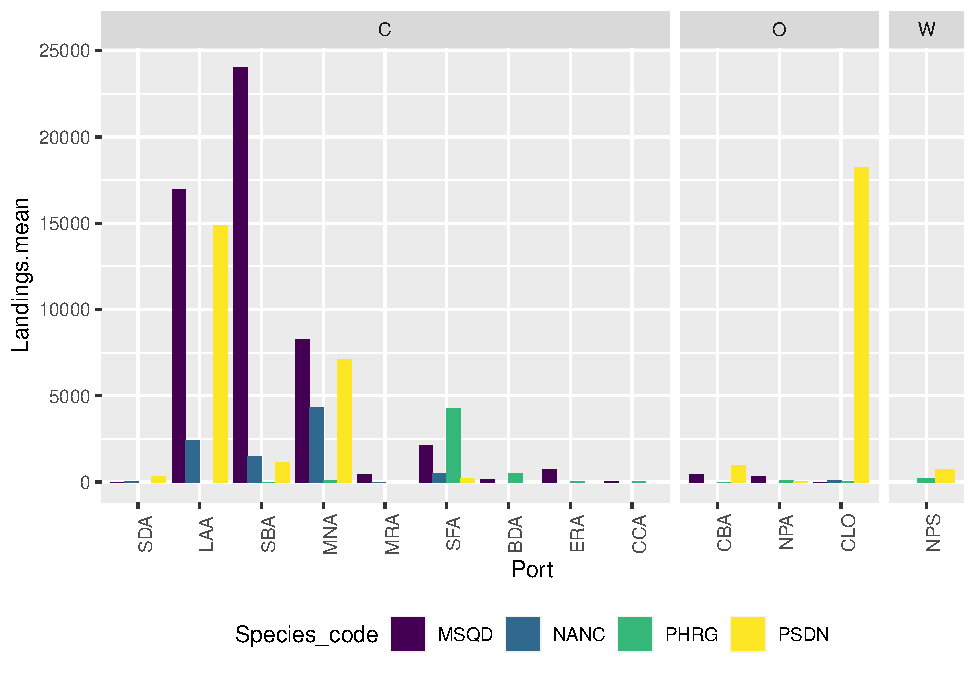
\includegraphics{econ_landings_paper_files/figure-latex/avg_landings_by_port-1} \caption{Annual average landings by port area.\label{fig:avg_landings_by_ports}}\label{fig:avg_landings_by_port}
\end{figure}
\end{Schunk}

To analyze substitution more in detail, we compute total annual landing
by port during 1980-2020 period (Figure \ref{fig:ts_landings_by_ports}).
There is a general conception that vessel that harvest Pacific sardine
switch to market squid when the conditions are favorable. However, we
can notice from Figure \ref{fig:ts_landings_by_ports} that landings of
market squid have been decreasing in the last five years. We would
expect that the closure of the Pacific sardine fishery would have switch
targeted species, but the graphs show some complementary instead of
substitution. Under this scenario is useful to ask to ask whether after
the closure, vessel that harvest Market squid left the fishery or
stayed. We show the number of vessels by species in Figure
\ref{fig:ts_n_vessels}.

\begin{Schunk}
\begin{figure}
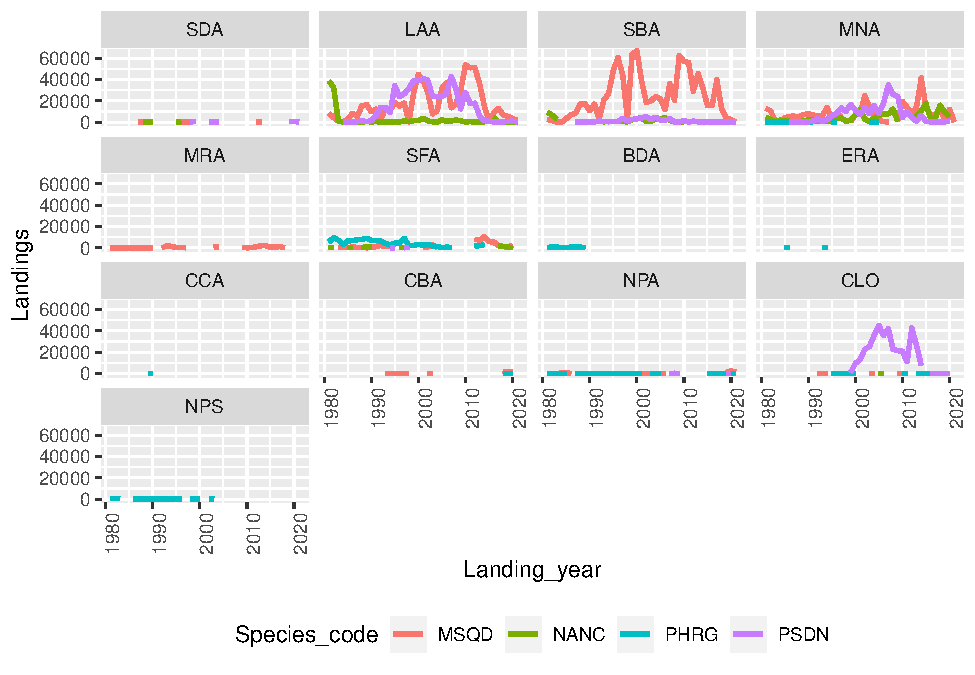
\includegraphics{econ_landings_paper_files/figure-latex/ts_by_port-1} \caption{Total annual landing by port area. 2000 - 2020. \textit{Notes:} CLO = Columbia River (OR); LAA = Los Angeles; MNA = Monterey; SBA = Santa Barbara; SFA = San Francisco.\label{fig:ts_landings_by_ports}}\label{fig:ts_by_port}
\end{figure}
\end{Schunk}

\begin{Schunk}
\begin{figure}
\includegraphics{econ_landings_paper_files/figure-latex/ts_n_vessels-1} \caption{Total number of vessel by species. 2000 - 2020.\label{fig:ts_n_vessels}}\label{fig:ts_n_vessels}
\end{figure}
\end{Schunk}

\hypertarget{methods}{%
\section{Methods}\label{methods}}

\hypertarget{data}{%
\subsection{Data}\label{data}}

Our data set contain a number of variables measured at the port and
\emph{vessel levels} for CPS the fishery located in the U.S. West Coast.
Our outcome variables are landings by port areas in a year and landing
by vessel in a month. These two different outcome variables would allows
us to study the degree of flexibility that vessel have in comparison to
ports in regard to species substitution and catch composition. If
vessels have strong contracts with processor associated with a port,
then we should observe that substitution of vessels and port is similar.
Yearly panel data data on landing by port areas during the the period
1980 - 2020 is publicly available from
\href{http://pacfin.psmfc.org/}{PacFIN}. \textbf{Vessel level data was
obtained upon request from\ldots{}} We only include ports areas where
substitution could happen. In practical terms, we drop port that have
never landed either Pacific sardine, market squid or Northern anchovy
during our period of analysis.\footnote{N/A were converted to zero.} We
assume that this criteria would allows to identify ports that have the
infrastructure to land all of the species in consideration.

Our main treatment variables are species probability of presence. This
variables were obtained from Species Distribution Models (SDM), and
future forecast of these variables allows us to simulate the CPS fishery
in the future. Prior landings models have shown that the probability of
presence have a large contribution on explaining landings. For instance,
\citet{smith2021potential} use mean monthly probability of presence of
sardine within 60 km of the port as explanatory variable. They found a
positive effect of probability of presence on Pacific sardine landings.
Moreover, landings where mostly explained by this variable. We follow
their same procedure to associate SDM's outputs with ports. For Pacific
sardine, we compute the average probability of presence within the same
radius of 60 kilometers around the port. This radious also coincide with
the average distance with two standard deviation traveled by vessels
based on logbook availables for this fisheries. For market squid and
Northern anchovy, we set this radius to 90 km. We also use logbook in
the case or market squid, while for the Northern anchovy, the optimal
distance for Northern anchovy was chosen empirically.\footnote{To see an
  animation of how far vessel travel please visit
  \href{https://drive.google.com/file/d/1-PE_lcZNcXNcyILA_6xhkHyEhV3mV2TA/view?usp=sharing}{this
  link}.}

Figure \ref{fig:sdm_land_by_port} show the relationship between the
probability of presence and landings by species in three main port
areas: Los Angeles, Monterrey and Santa Barbara areas. The graph suggest
that Pacific sardine landings are positive correlated with the
probability of presence of this species, similar to
\citet{smith2021potential}. This is also true in Monterrey area for the
Northern anchovy, In the case of market squid, we cannot distinguish
correlation between landings and probability of presence. Note, however,
that the evidence shown in this figure may not capturing the actual
effect of the probability of presence as other effect may be in play.
Our empirical strategy is designed to isolate the effect of the
probability on landing in a multivariate model framework.

\begin{Schunk}
\begin{figure}
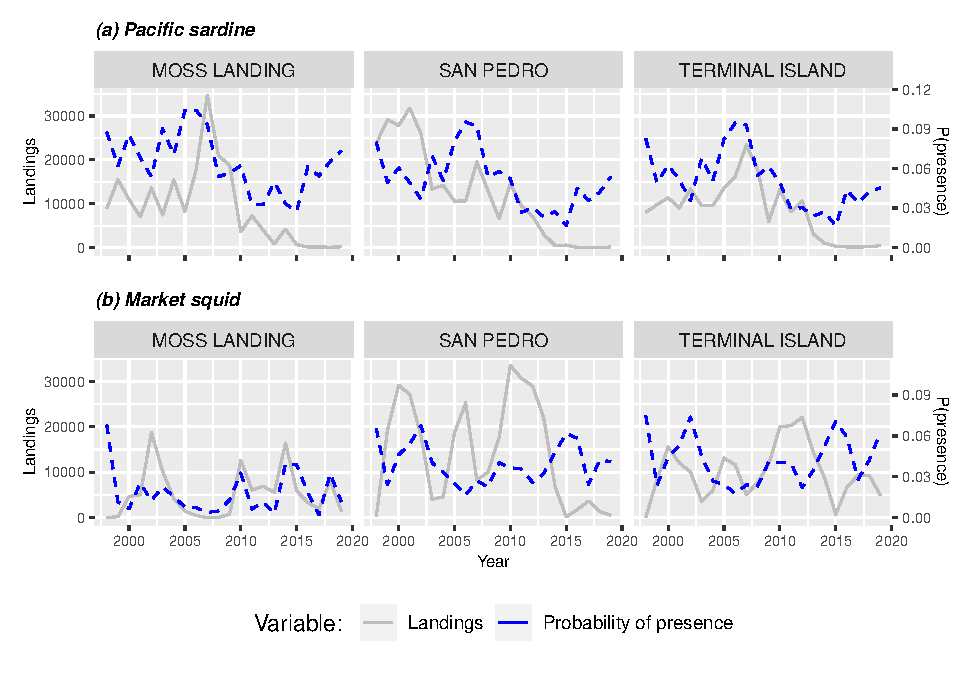
\includegraphics{econ_landings_paper_files/figure-latex/SDM_land_by_port-1} \caption{Landings v/s probability of presence by port area. \textit{Notes:} LAA = Los Angeles; MNA = Monterey; SBA = Santa Barbara.\label{fig:sdm_land_by_port}}\label{fig:SDM_land_by_port}
\end{figure}
\end{Schunk}

Beside the biological stock, landings are affected by socio-economics
conditions. Some of them are harvest cost, prices received by species
and their substitutes, and regulations imposed by the authorities. In
our data we include as a proxy of harvest cost average distances
traveled by vessel from the port of origin \emph{(TO BE INCLUDED USING
GLOBAL FISHING WATCH\ldots)} and fuel cost \emph{(TO BE
INCLUDED\ldots)}. Own price was included and it was obtained from PacFIN
landings dataset. When price was missing, we replace this value for the
average price of the species in all ports for the corresponding year. We
include the Annual Catch Limit (ACL) for the Pacific sardine model. The
ACL for Pacific sardine were obtained from the \href{pcouncil.org}{CPS
Fisheries Management Plan}???. A summary statistics of our data set is
shown in Table \ref{tab:sum_stats}.

\begin{table}[!htbp] \centering \renewcommand*{\arraystretch}{1.1}\caption{Summary Statistics \label{tab:sum_stats}}\resizebox{\textwidth}{!}{
\begin{tabular}{lrrrrrrr}
\hline
\hline
Variable & N & Mean & Std. Dev. & Min & Pctl. 25 & Pctl. 75 & Max \\ 
\hline
Landings: PSDN & 92 & 10828.886 & 13499.627 & 0.1 & 156.025 & 20991.3 & 45016.5 \\ 
Landings: MSQD & 103 & 13383.623 & 17166.411 & 0.1 & 222.2 & 19693.75 & 66890.3 \\ 
Landings: NANC & 59 & 2769.698 & 3928.055 & 0 & 149.55 & 3651.65 & 17180.2 \\ 
Prob(presence): PSDN & 322 & 0.261 & 0.104 & 0.08 & 0.177 & 0.341 & 0.569 \\ 
Prob(presence): MSQD & 280 & 0.17 & 0.078 & 0.025 & 0.12 & 0.217 & 0.467 \\ 
Prob(presence): NANC & 308 & 0.306 & 0.153 & 0.085 & 0.181 & 0.39 & 0.846 \\ 
Price: PSDN & 437 & 0.079 & 0.039 & 0 & 0.05 & 0.108 & 0.37 \\ 
Price: MSQD & 437 & 0.266 & 0.121 & 0 & 0.185 & 0.32 & 0.5 \\ 
Price: NANC & 437 & 0.091 & 0.054 & 0 & 0.06 & 0.114 & 0.35 \\ 
Revenue: PSDN & 92 & 1497414 & 1920819.177 & 0 & 31471 & 2646660.75 & 8979099 \\ 
Revenue: MSQD & 103 & 7734746.485 & 9938728.985 & 0 & 97348 & 11193641.5 & 43742173 \\ 
Revenue: NANC & 59 & 311373.814 & 427339.961 & 17 & 42203 & 437046.5 & 1930490 \\ 
Annual Catch Limit: PSDN & 436 & 82613.151 & 55614.651 & 0 & 30259 & 122747 & 186791\\ 
\hline
\hline
\end{tabular}
}
\end{table}

\hypertarget{empirical-model}{%
\subsection{Empirical model}\label{empirical-model}}

We use a Hierarchical Bayesian Hurdle model to estimate the effect of
species distribution on fish landings. We estimate a separate model for
the three species in consideration. We use a Bayesian framework for
several reasons. First, it allows us to consider uncertainty from
modeling the process as well as from the imperfect observation of the
process, assuming that all parameters are random variables. Second, it
allows us to incorporate multilevel effects (i.e.~hierarchical effects).
Finally, it allow us to incorporate previous knowledge as a prior. For
instance, we can include a prior the results obtained in
\citet{smith2021potential} for the Pacific sardine landing equation.

Specifically, we fit a hierarchical Bayesian hurdle model to model the
zeros included in our landing data. We observe a zero when no landings
occur in a specific time period (landings observations with ``NA'' were
transformed to zero). This zero could mean that there was no incentives
for the fleet/vessel to harvest the species in consideration. In
general, our Bayesian models have the following structure:
\begin{align*}
[\theta_i | q_{i,t}] &  \varpropto f\left(q_{i,t} | \theta_i\right) \times [\theta_i] 
\end{align*} where \(q_{i,t}\) is the observed landings of the
corresponding species in port \(i \in (1,\ldots,L)\) at year \(t\),
\(L\) is the total number of port, and \(\theta_i\) are the parameters
(i.e.~random-coefficients) to be estimated at the port level. The latter
give the name of hierarchical to our model.\footnote{For more details
  about Hierarchichal models, see \cite{hobbs2015}.} The distribution
\(f\left(q_{i,t} | \theta_j\right)\) can be rewritten as:
\begin{equation}
f\left(q_{i,t} | \theta_j \right) = \begin{cases}
p_i & \text{if} \quad q_{it} = 0  \\ 
\left[1-p_i\right] \text{gamma} \left(q_{i,t} | \frac{\mu^2}{\sigma^2}, \frac{\mu}{\sigma^2} \right) & \text{if} \quad q_{it} > 0. 
\end{cases}
\end{equation} where \(\text{logit}(p_{i,j}) = \bf{X}\gamma\) and
\(\mu = \bf{X}\beta\). Specifically \(\mu\) is defined as the following:
\begin{equation}
\mu_{i,j} = \beta_{0,i} + \beta_{1,j} P(Precense)_{PSDN} + \beta_{2,j} + P(Precense)_{MSQD} + \beta_{3,j} P(Precense)_{NANC}.
\end{equation} where \(j\) indicate the species in consideration.
\(\text{logit}(p_{i,j})\) follows the same structure, but coefficient
are replaced by \(\gamma\).

For the Pacific sardine, we also include annual catch limits as an
additional explanatory variable in both \(\mu_i\) and
\(\text{logit}(p_i)\) equations. We restrict our data set for this
species to the period when the fishery was open (2000-2015). We only
consider ports where landing have occur at least once in our sample
period. Thus, we avoid to deal with ports where infrastructure to land
Pacific sardine is inexistent.

In the case of market squid, our databse comprise the time period
between 2000 and 2018. We do not include ACL as an explanatory variable
as there is no variation between years. To capture any change on fishers
behavior when Pacific sardine fishery closed, we include a binary
variable called \textbf{dClose} that takes the value ``1'' when the
Pacific sardine fishery is close, and the value ``0'' when its close.
Pacific sardine probability takes the value of zero when the fishery is
closed. Thus, the effect of this variable is only relevant when it
PAcific sardine fishery is open in order to capture potential
substitution between targets.

Finally, a similar structure than Market squid models is followed for
our estimation of Northern anchovy landing by ports.

\hypertarget{results}{%
\section{Results}\label{results}}

\hypertarget{graphical-posterior-predictive}{%
\subsection{Graphical posterior
predictive}\label{graphical-posterior-predictive}}

Before presenting the results for the three species in consideration, we
check graphically whether the posterior distribution is able to predict
the actual distribution. We exclude zero in our graph to avoid plotting
different data generation processes. In Figure \ref{fig:posteriors} we
show a posterior sample compare with the true sample distribution for
the three species in analysis. Some deviation from the true sample
distribution is observed in the three models, but still the posterior
sample follow a similar shape than the actual curve. Moreover, our
pacific sardine sample do well in predicting probabilities at lower
landing levels.

\begin{Schunk}
\begin{figure}
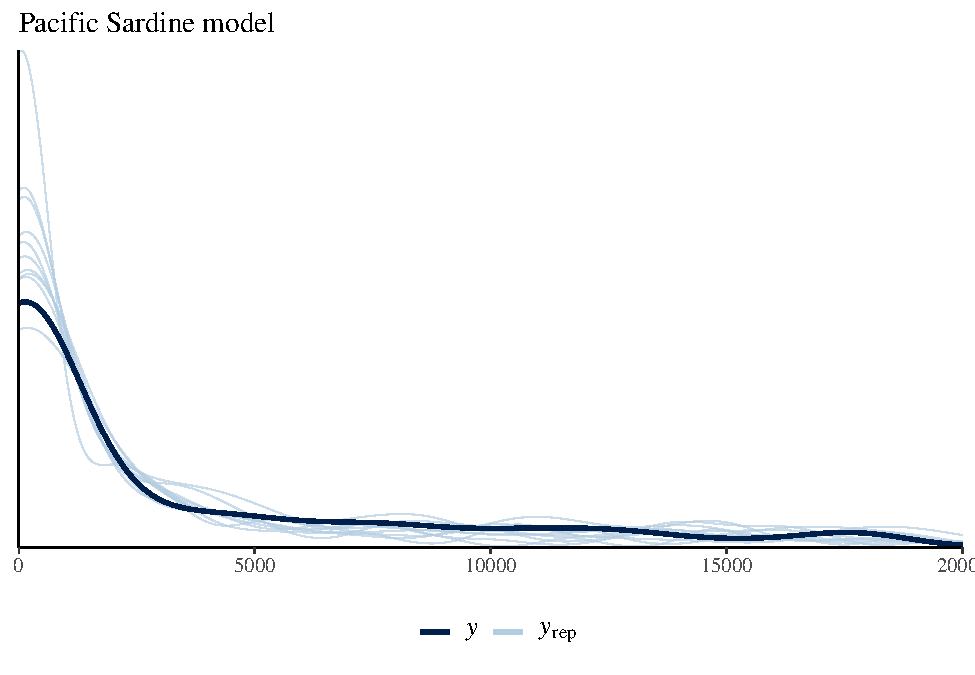
\includegraphics{econ_landings_paper_files/figure-latex/y_rep-1} \caption{Graphical posterior predictive checks\label{fig:posteriors}}\label{fig:y_rep}
\end{figure}
\end{Schunk}

In addition to a posterior predictive check, we also check divergence
and treedepth.\footnote{Explain what are these concepts\ldots{}} In all
three models, we did not have any divergent step in our estimation. The
maximum treedepth was 11 for the Pacific sardine model, while in the
other it was 10.

\hypertarget{own-species-distribution-effect}{%
\subsection{Own species distribution
effect}\label{own-species-distribution-effect}}

The inclusion of hierarchical effects by port allows us to analyze the
effects of the probability of presence on landings disaggregated by
ports.

\begin{Schunk}
\begin{figure}
\includegraphics{econ_landings_paper_files/figure-latex/by_port_sdm-1} \caption{Effect of probability of presence on landings by species and port\label{fig:sdmeffects}}\label{fig:by_port_sdm}
\end{figure}
\end{Schunk}

\hypertarget{interaction-effects}{%
\subsection{Interaction effects}\label{interaction-effects}}

\begin{Schunk}
\begin{figure}
\includegraphics{econ_landings_paper_files/figure-latex/int_effect_PSDN_by_port_PLOT-1} \caption{Interaction effects between species distribution on Pacific sardine landings by port\label{fig:sdm_int_psdn}}\label{fig:int_effect_PSDN_by_port_PLOT}
\end{figure}
\end{Schunk}

\begin{Schunk}
\begin{figure}
\includegraphics{econ_landings_paper_files/figure-latex/int_effect_MSQD_by_port_PLOT-1} \caption{Interaction effects between species distribution on market squid landings by port\label{fig:sdm_int_msqd}}\label{fig:int_effect_MSQD_by_port_PLOT}
\end{figure}
\end{Schunk}

\begin{Schunk}
\begin{figure}
\includegraphics{econ_landings_paper_files/figure-latex/int_effect_NANC_by_port_PLOT-1} \caption{Interaction effects between species distribution on Northern anchovy landings by port\label{fig:sdm_int_nanc}}\label{fig:int_effect_NANC_by_port_PLOT}
\end{figure}
\end{Schunk}

\hypertarget{pacific-sardine-closure}{%
\subsection{Pacific sardine closure}\label{pacific-sardine-closure}}

\begin{Schunk}
\begin{figure}
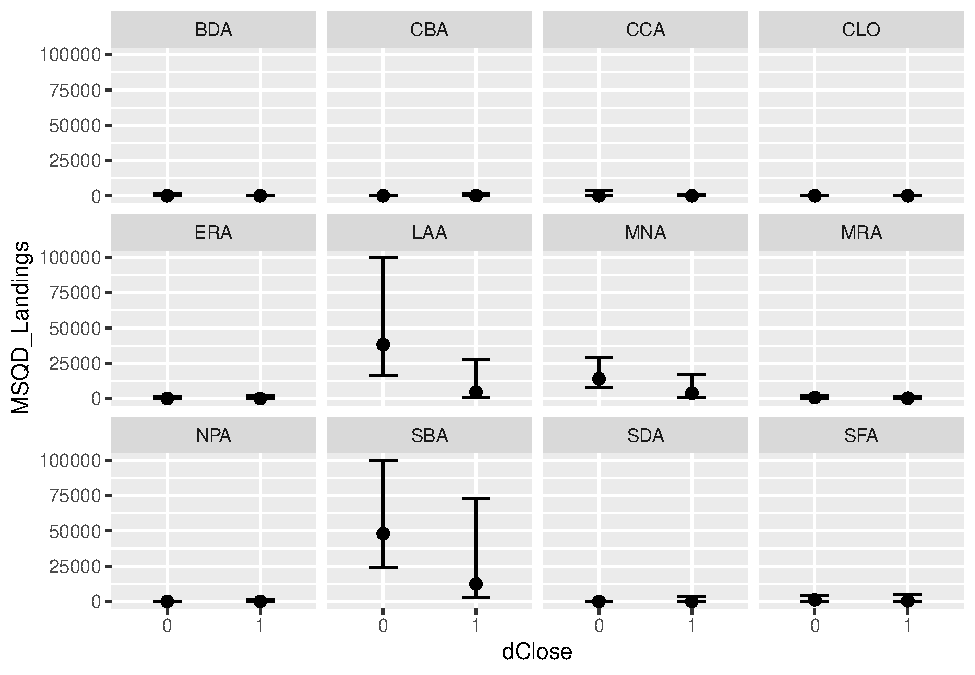
\includegraphics{econ_landings_paper_files/figure-latex/by_port_msqd_dclose-1} \caption{Effect of Pacific sardine fishery closure on markt squid landings by species and  port\label{fig:sdmeffects}}\label{fig:by_port_msqd_dclose}
\end{figure}
\end{Schunk}

\hypertarget{predictions}{%
\section{Predictions}\label{predictions}}

\ldots{}

\hypertarget{conclusions}{%
\section{Conclusions}\label{conclusions}}

A possible extension of our research is to consider spatial
autocorrelations between ports.\footnote{See \cite{morris2019bayesian}
  for an application of a spatial model in a Bayesian framework.} Ports
landing maybe correlated as vessel have the incentives to choose the
port of landing, conditional on whether the port have the infrastructure
for this. It is likely that they just land wherever is closer to the
area they are fishing. Nevertheless, differential in prices could
encourage them to travel a little further for higher prices.

\bibliography{econ-landings-paper.bib}

\address{%
Author One\\
Affiliation\\%
line 1\\ line 2\\
%
\url{https://journal.r-project.org}\\%
\textit{ORCiD: \href{https://orcid.org/0000-0002-9079-593X}{0000-0002-9079-593X}}\\%
\href{mailto:author1@work}{\nolinkurl{author1@work}}%
}

\address{%
Author Two\\
Affiliation 1\\%
line 1 affiliation 1\\ line 2 affiliation 1\\
Affiliation 2\\%
line 1 affiliation 2\\ line 2 affiliation 2\\
%
\url{https://journal.r-project.org}\\%
\textit{ORCiD: \href{https://orcid.org/0000-0002-9079-593X}{0000-0002-9079-593X}}\\%
\href{mailto:author2@work}{\nolinkurl{author2@work}}%
}

\address{%
Author Three\\
Affiliation\\%
line 1 affiliation\\ line 2 affiliation\\
%
\url{https://journal.r-project.org}\\%
%
\href{mailto:author3@work}{\nolinkurl{author3@work}}%
}
